% =============================================================================

\vspace*{\fill}

\begin{figure}[!h]
\begin{lstlisting}[language=pseudo,style=block]
saes.v1.encs rd, rs1 : v1.SubBytes(rd, rs1, fwd=1)
saes.v1.decs rd, rs1 : v1.SubBytes(rd, rs1, fwd=0)
saes.v1.encm rd, rs1 : v1.MixColumn(rd, rs1, fwd=1)
saes.v1.decm rd, rs1 : v1.MixColumn(rd, rs1, fwd=0)
\end{lstlisting}
\caption{
  Instruction mnemonics, and their mapping onto pseudo-code functions, for \ISE{1}.
}
\label{fig:v1:mnemonics}
\end{figure}

\begin{figure}[!h]
\begin{lstlisting}[language=pseudo,style=block]
v1.SubByte(rd, rs1, fwd):
    rd.8[i] = AESSBox[rs1.8[i]] if fwd else AESInbSBox[rs1.8[i]] for i=0..3

v1.MixColumn(rd, rs1, fwd)
    for i=0..3:
        tmp.32  = ROTL32(rs1.32, 8*i)
        rd.8[i] = AESMixColumn(tmp.32) if fwd else AESInvMixColumn(tmp.32)
\end{lstlisting}
\caption{
  Instruction pseudo-code functions for \ISE{1}.
}
\label{fig:v1:pseudo}
\end{figure}

\begin{figure}[!h]
\begin{lstlisting}[language=pseudo,style=block]
lw           a0,  0(a4)       // Load Round Key
lw           a1,  4(a4)
lw           a2,  8(a4)
lw           a3, 12(a4)
xor          a4, a4, a0       // Add Round Key
xor          a5, a5, a1
xor          a6, a6, a2
xor          a7, a7, a3
saes.v1.encs a0, a4           // SubBytes
saes.v1.encs a1, a5
saes.v1.encs a2, a6
saes.v1.encs a3, a7
                              // Shift Rows
and          a4, t0, t6   ; and   a5, t1, t6
and          a6, t2, t6   ; and   a7, t3, t6
slli         t4, t6, 0x8  ; and   t5, t0, t4
or           a7, a7, t5   ; and   t5, t3, t4
or           a6, a6, t5   ; and   t5, t2, t4
or           a5, a5, t5   ; and   t5, t1, t4
or           a4, a4, t5   ; slli  t4, t4, 0x8
and          t5, t2, t4   ; or    a4, a4, t5
and          t5, t3, t4   ; or    a5, a5, t5
and          t5, t0, t4   ; or    a6, a6, t5
and          t5, t1, t4   ; or    a7, a7, t5
slli         t4, t4, 0x8  ; and   t5, t3, t4
or           a4, a4, t5   ; and   t5, t0, t4
or           a5, a5, t5   ; and   t5, t1, t4
or           a6, a6, t5   ; and   t5, t2, t4
or           a7, a7, t5
saes.v1.encm t0, a4           // MixColumns
saes.v1.encm t1, a5
saes.v1.encm t2, a6
saes.v1.encm t3, a7
\end{lstlisting}
\caption{
  An AES encryption round implemented using \ISE{1}.
}
\label{fig:v1:round}
\end{figure}

\vspace*{\fill}

% -----------------------------------------------------------------------------

\newpage

\vspace*{\fill}

\begin{figure}[!h]
\centering
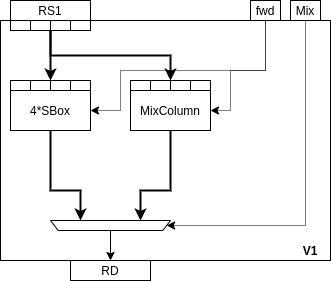
\includegraphics[width={0.5\textwidth}]{diagrams/ise-datapath-v1.png}
\caption{
  A diagrammatic description of the functional unit required to support \ISE{1}.
}
\label{fig:v1:fu}
\end{figure}

\vspace*{\fill}

% =============================================================================
